\documentclass[12pt,a4paper]{article}

\usepackage[left=3cm, right=3cm, top=2.5cm, bottom=2.5cm, headheight=38.40865pt]{geometry} % Adjusted headheight
\usepackage{setspace}
\usepackage{amsmath}
\usepackage{tikz}
\usepackage{pgfplotstable}
\usepackage{titlesec}
\usepackage{bm}
\usepackage{tcolorbox}
\tcbuselibrary{skins}
\usepackage{empheq}
\usepackage{booktabs}
\usepackage{caption}
\usepackage{hyperref}
\usepackage{fancyhdr}
\usepackage{float}
\usepackage{silence}
\WarningFilter{caption}{The option `hypcap=true' will be ignored}
\hypersetup{
    colorlinks=true,
    linkcolor=black,
    filecolor=magenta,      
    urlcolor=cyan,
    pdfpagemode=FullScreen,
    }
\usepackage{graphicx}
\graphicspath{ {./images/} }

\pgfplotsset{compat=1.18}

\titleformat{\section}{\Large\bfseries}{\thesection}{1em}{}
\titleformat{\subsection}{\large\bfseries}{\thesubsection}{1em}{}

\renewcommand{\contentsname}{Table des Matières}
\renewcommand{\tablename}{Tableau}

\title{Force de Laplace}
\author{Liviu Arsenescu, Cătălin Bozan}
\date{23.04.2024}

\newtcbox{\mymath}[1][]{%
    nobeforeafter,
    tcbox raise base,
    enhanced,
    colframe=black,
    colback=white,
    boxrule=1pt,
    drop shadow={
        xshift=3pt, % Removed 'shadow' prefix
        yshift=-3pt, % Removed 'shadow' prefix
        opacity=1
    },
    #1
}

\pagestyle{fancy}
\fancyhf{}
\rhead{
\includegraphics[width=4cm]{hearclogo.png}}
\lhead{\thepage}
\setlength{\headsep}{30pt}

\begin{document}
    \pagenumbering{gobble}
    \begin{titlepage}
        \begin{center}
            \vspace*{\fill}
            \Huge \textbf{Force de Laplace} \\
            \Huge \textbf{Étude du champ magnétique} \\
            \Large Rapport du Laboratoire \\
            \begin{figure}[h]
                \centering
                
\includegraphics[width=7cm]{hearclogo.png}
            \end{figure}
            \vspace{\fill}
            \Large Liviu Arsenescu, Cătălin Bozan \\
            23.04.2024

            \vspace*{\fill}
        \end{center}
    \end{titlepage}

    \thispagestyle{empty}
    \tableofcontents
    \newpage

    \pagenumbering{arabic}
    \section{Description de l'expérience}
    \subsection{Buts}
    \begin{itemize}
        \item Étude de la force de Laplace
        \item Démontrer la dépendance linéaire de la force par rapport au champ magnétique $\bm{B}$
    \end{itemize}

    \subsection{Éléments théoriques}
    \subsubsection{Les différentes grandeurs physiques rencontrées}
    \begin{minipage}{0.6\linewidth}
        \begin{itemize}
            \item $\bm{F_L}$ - force de Laplace
            \item $\bm{P}$ et $\bm{N}$ - force du poids et force normale
            \item $\bm{I}$ - courant électrique
            \item $\bm{l}$ - longueur du conducteur
            \item $\bm{\theta}$ - l'angle entre les vecteurs $I \vec{l}$ et $\vec{B}$
            \item $\bm{m}$ - différentes masses
            \item $\bm{g}$ - l'accélération gravitationnelle de la Terre
        \end{itemize}
    \end{minipage}%
    \hfill
    \begin{minipage}{0.4\linewidth}
        \begin{itemize}
            \item[-] $\bm{[ceva]=unitate}$
        \end{itemize}   
    \end{minipage}

    \subsubsection{Modèle Théoriques}
    Pour décrire le modèle mathématique dont on a besoin, on partira de la formule suivante : 
    \begin{empheq}[box={\mymath}]{equation*}
        \vec{F_L} = I \vec{l} \times \vec{B}
    \end{empheq}
    Comme on le sait, la norme d'un vecteur résultant d'un produit vectoriel peut être écrit comme suit :
    \begin{equation*}
        ||\vec{F_L}|| = ||I \vec{l}|| \cdot ||\vec{B}|| sin(\theta) \Rightarrow ||\vec{F_L}|| = IlBsin{\theta} 
    \end{equation*}

    Pour la configuration de la bobine, on peut représenter les forces agissant comme suit :
    \begin{figure}[H]
        \centering
        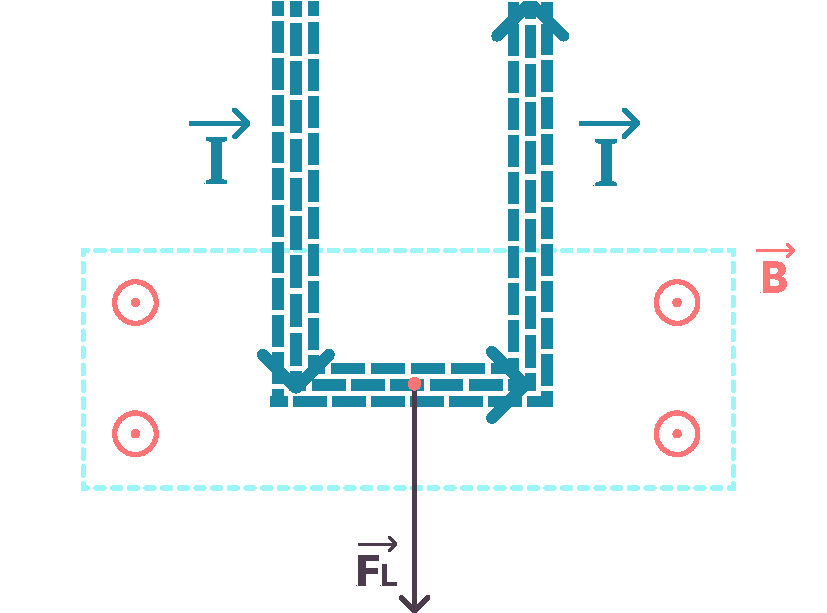
\includegraphics[scale=0.5]{images/magnet_coil.pdf}
        \caption{Système de forces de la bobine}
    \end{figure}
    En utilisant la troisième loi de Newton, on peut construire le système de forces suivant sur l'aimant :
    \begin{figure}[H]
        \centering
        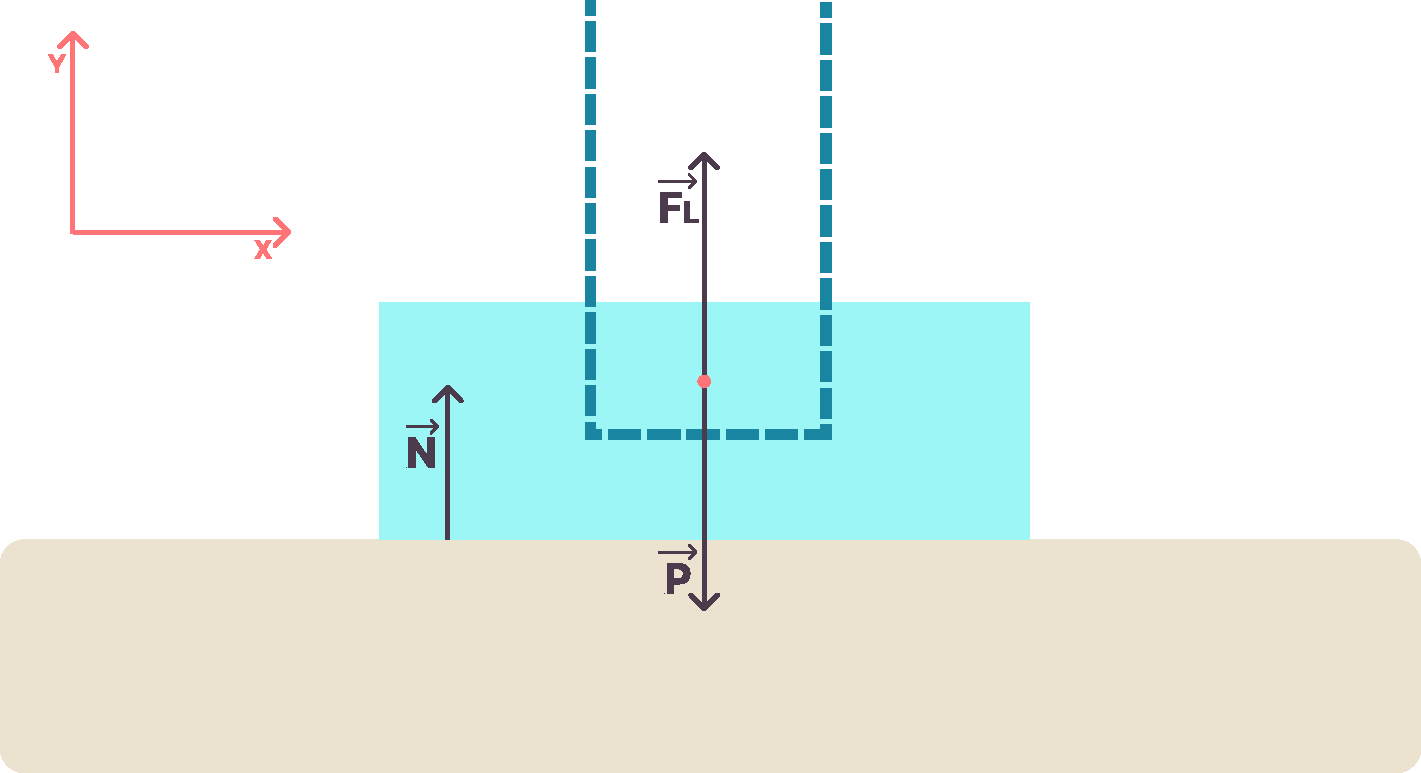
\includegraphics[scale=0.5]{images/magnet_side.pdf}
        \caption{Système de forces sur l'aimant}
    \end{figure}
    En utilisant la deuxième loi de Newton dans la dernière figure, on obtient :
    \begin{equation*}
        \Sigma \vec{F} = 0 \Rightarrow \vec{F_L} + \vec{N} + \vec{P} = 0
    \end{equation*}
    On observe que les forces agissent uniquement sur l'axe y, ce qui permet de déduire l'équation suivante :
    \begin{equation*}
        \pm F_L + N - P = 0
    \end{equation*}
    En alimentant la bobine en courant, on constate que deux masses différentes apparaissent sur la balance :
    \begin{itemize}
        \item $m_0$ - masse de l'aimant
        \item $m_1$ - masse apparente de l'aimant
    \end{itemize}
    Avec ces deux mesures, on peut développer à nouveau l'équation :
    \begin{align*}
        \pm F_L + m_1g - m_0g &= 0 \\
        |F_L| &= |m_1 - m_0|g \\
        |F_L| &= \delta m g
    \end{align*}
    Où $\delta m$ est le module de la différence entre $m_1$ et $m_0$. \\
    Égalant ce que on a obtenu pour $||\vec{F_L}||$ et pour $|F_L|$, on obtient :
    \begin{equation*}
        \left.
        \begin{aligned}
            |F_L| &= \delta mg \\
            ||\vec{F_L}|| &= IlB\sin(\theta)
        \end{aligned}
        \right\}
        \Rightarrow
        \delta mg = \frac{IlBsin(\theta)}{g}
    \end{equation*}
    On peut donc conclure que $\delta m$ est une fonction qui dépend de $I$, $l$, $B$, $sin(\theta)$.

    \subsection{Principe de l'expérience}
    \sloppy
    Comme indiqué ci-dessus, l'expérience consiste à calculer la valeur du champ magnétique $B$ par trois méthodes différentes :
    \begin{itemize}
        \item On va mesurer la pente de la fonction $\delta m$ en faisant varier uniquement le courant $I$, ce qui nous permettra de calculer $B$.
        \item On va mesurer la pente de la fonction $\delta m$ en faisant varier uniquement l'angle $\theta$, d'où on peut calculer de la même façon $B$.
        \item On mesure $B$ à l'aide d'un teslamètre.
    \end{itemize}

    \subsection{Schéma et montage de l’expérience}
    Pour réaliser l'expérience, on doit faire un dispositif qui nous permettre de générer la force de Laplace sur un aimant. On a donc : 
    \begin{figure}[H]
        \begin{minipage}{0.45\linewidth} % Adjusted width
            \begin{itemize}
                \item Une source de courant continu
                \item Un ampèremètre
                \item Un socle
                \item Une tige
                \item Un noix double
                \item Une bobine à \\
                    orientation réglable
                \item Un aimant en U
                \item Une balance
                \item Trois câbles de connexion
                \item Un teslamètre
                \item Une règle
            \end{itemize}
        \end{minipage}%
        \hfill
        \begin{minipage}{0.5\linewidth} % Adjusted width
            \centering
            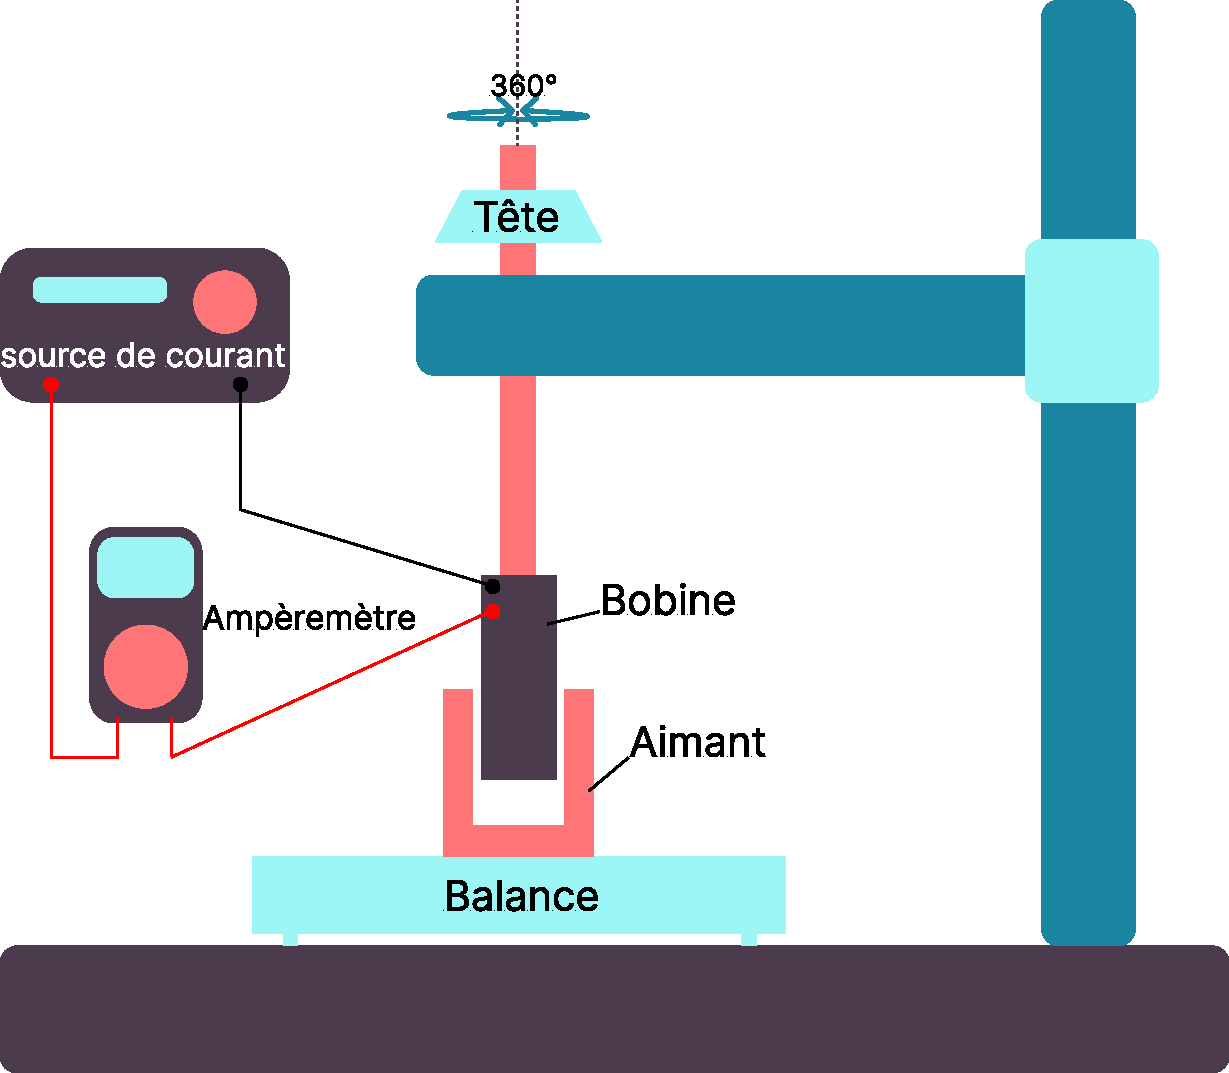
\includegraphics[scale=0.35]{images/experiment_layout.pdf}
            \caption{Système de forces de la bobine}
        \end{minipage}
    \end{figure}

    \subsection{Déroulement de l'expérience}
    \subsubsection{Étalonnage bobine-aimant}
    \begin{itemize}
        \item On met l'aimant sur la balance
        \item On fixe la bobine réglable sur le support
        \item On connecte la bobine en série avec l'ampèremètre à la source de courant
        \item En utilisant la tête rotative, on fixe la bobine de manière à ce que la force de Laplace soit nulle, et on considère cette angle comme $\theta = 0$\textdegree
    \end{itemize}
    \subsubsection{Force de Laplace en fonction du courant \textit{I}}
    \begin{itemize}
        \item On règle l'angle de la bobine a 90\textdegree, et on lui donne un courant de 4A
        \item On mesure $\delta m$ pour des valeurs de $I$, par intervalles de 0,4A, de 4A à 0A
    \end{itemize}
    \subsubsection{Force de Laplace en fonction de l'angle \texorpdfstring{$\theta$}{theta}}
    \begin{itemize}
        \item On fixe le courant à 4A, et on ramène la bobine à 0\textdegree
        \item On mesure $\delta m$ pour des valeurs de $\theta$ de 5 en 5, de 90\textdegree à 0\textdegree
    \end{itemize}
    \subsubsection{En utilisant le teslamètre}
    \begin{itemize}
        \item On place la sonde du teslamètre dans la zone entre les pôles de l'aimant, puis on mesure le champ magnétique $B$
    \end{itemize}

    \section{Mesures}
    \subsection{Mesures constantes :}
    \begin{itemize}
        \item $L = (0.010 \pm 0.001)$ m - longueur de la section de la bobine
        \item $n = 11$ - nombre de spires
        \item $m_0 = (70.40 \pm 0.01)$ g - masse de l'aimant
        \item $\Delta I = \pm 0.01$ A - incertitude sur le courant électrique
        \item $\Delta \theta = \pm 2$\textdegree - incertitude de l'angle
        \item $B_3 = -43.3$ mT - champ magnétique mesuré avec le teslamètre
        \item $\Delta B_3 = \pm 0.4$ mT - incertitude du champ magnétique
    \end{itemize}
    \subsection{Tableaux des mesures :}
    \subsubsection{\textit{I} variable}
    \begin{minipage}{0.4\textwidth}
        \centering
        \begin{tabular}{c|c|c}
            \toprule
            $I$(A) & $\delta m$(g) & $\Delta(\delta m)$(g) \\
            \midrule
            0.41 & -0.12 & 0.02 \\
            0.81 & -0.33 & 0.02 \\
            1.20 & -0.56 & 0.02 \\
            1.60 & -0.77 & 0.02 \\
            2.01 & -1.01 & 0.02 \\
            2.40 & -1.22 & 0.02 \\
            2.81 & -1.46 & 0.02 \\
            3.21 & -1.68 & 0.02 \\
            3.61 & -1.90 & 0.02 \\
            4.01 & -2.13 & 0.02 \\
            \bottomrule
        \end{tabular}
        \captionof{table}{$I$ variable}
    \end{minipage}%
    \hfill
    \begin{minipage}{0.6\textwidth}
        Légende :
        \begin{itemize}
            \item $I$ - courant électrique (en A)
            \item $\delta m$ - différence entre les masses $m_1$ et $m_0$ (en g)
            \item $\Delta(\delta m)$ - incetitude de $\delta m$ (en g)
        \end{itemize}
    \end{minipage}
    \subsubsection{\texorpdfstring{$\theta$}{theta} variable}
    \begin{minipage}{0.4\textwidth}
        \centering
        \begin{tabular}{c|c|c}
            \toprule
            $\theta$(\textdegree) & $\delta m$(g) & $\Delta(\delta m)$(g) \\
            \midrule
            0  &  0.09 & 0.02 \\
            5  & -0.10 & 0.02 \\
            10 & -0.30 & 0.02 \\
            15 & -0.49 & 0.02 \\
            20 & -0.66 & 0.02 \\
            25 & -0.85 & 0.02 \\
            30 & -1.01 & 0.02 \\
            35 & -1.17 & 0.02 \\
            40 & -1.33 & 0.02 \\
            45 & -1.46 & 0.02 \\
            50 & -1.58 & 0.02 \\
            55 & -1.69 & 0.02 \\
            60 & -1.79 & 0.02 \\
            65 & -1.88 & 0.02 \\
            70 & -1.94 & 0.02 \\
            75 & -2.00 & 0.02 \\
            80 & -2.03 & 0.02 \\
            85 & -2.06 & 0.02 \\
            90 & -2.13 & 0.02 \\
            \bottomrule
        \end{tabular}
        \captionof{table}{$\theta$ variable}
    \end{minipage}%
    \hfill
    \begin{minipage}{0.6\textwidth}
        Légende :
        \begin{itemize}
            \item $\theta$ - l'angle entre les vecteurs $I \vec{l}$ et $\vec{B}$ (en degrées)
            \item $\delta m$ - différence entre les masses $m_1$ et $m_0$ (en g)
            \item $\Delta(\delta m)$ - incetitude de $\delta m$ (en g)
        \end{itemize}
    \end{minipage}

    \section{Analyse des mesures et résultats}
    Pour calculer le champ magnétique $B$ en faisant varier le courant ou l'angle, on construit une régression linéaire à l'aide de la formule suivante :
    \begin{empheq}[box={\mymath}]{equation*}
        \delta m = \frac{IlBsin(\theta)}{g}
    \end{empheq}
    $l$ est la longueur du conducteur, donc $l = nL = (0.110 \pm 0.001)$ m.
    \subsection{\texorpdfstring{$\delta m$}{delta m} en fonction du courant \textit{I}}
    \pgfplotstableread[col sep=comma]{data/plot_I.csv}\plotIdata
    \begin{figure}[H]
        \centering
        \begin{tikzpicture}[scale=0.8]
            % Scatter plot
            \begin{axis}[
                xlabel={$I$ (A)},
                ylabel={$\delta m$ (g)},
                legend pos=north east,
                legend style={at={(0.25,0.05)}, anchor=south},
                grid=both,
                width=1\textwidth,
                height=0.3\textheight,
                x tick label style={
                    /pgf/number format/.cd,
                    precision=2,
                    fixed,
                    fixed zerofill,
                },
                y tick label style={
                    /pgf/number format/.cd,
                    precision=2,
                    fixed,
                    fixed zerofill,
                },
                xmin=0,
                xmax=4.5,
                ymin=-2.5,
                ymax=-0,
            ]
                \addplot+[only marks, mark=x, error bars/.cd, x dir=both, x explicit, y dir=both, y explicit] table[x=I, x error=err_I, y=dm, y error=err_dm] {\plotIdata};

                % Linear regression line
                \addplot [red, thick] table[
                    y={create col/linear regression={y=dm}}
                ] {\plotIdata};
                \xdef\slope{\pgfplotstableregressiona}
                \xdef\intercept{\pgfplotstableregressionb}

                % Add the equation of the line
                \addlegendentry{Données}
                \addlegendentry{Régr. Lin.: $y = \pgfmathprintnumber{\slope}x + \pgfmathprintnumber{\intercept}$}
            \end{axis}
        \end{tikzpicture}
    \end{figure}
    \subsection{\texorpdfstring{$\delta m$}{delta m} en fonction de l'angle \texorpdfstring{$\theta$}{theta}}
    \pgfplotstableread[col sep=comma]{data/plot_T.csv}\plotTdata
    \begin{figure}[H]
        \centering
        \begin{tikzpicture}[scale=0.8]
            % Scatter plot
            \begin{axis}[
                xlabel={$sin(\theta)$},
                ylabel={$\delta m$ (g)},
                legend pos=north east,
                legend style={at={(0.3,0.05)}, anchor=south},
                grid=both,
                width=1\textwidth,
                height=0.3\textheight,
                x tick label style={
                    /pgf/number format/.cd,
                    precision=2,
                    fixed,
                    fixed zerofill,
                },
                y tick label style={
                    /pgf/number format/.cd,
                    precision=2,
                    fixed,
                    fixed zerofill,
                },
                xmin=-0.1,
                xmax=1.1,
                ymin=-2.5,
                ymax=-0,
            ]
                \addplot+[only marks, mark=x, error bars/.cd, x dir=both, x explicit, y dir=both, y explicit] table[x=T, x error=err_T, y=dm, y error=err_dm] {\plotTdata};

                % Linear regression line
                \addplot [red, thick] table[
                    y={create col/linear regression={y=dm}}
                ] {\plotTdata};
                \xdef\slope{\pgfplotstableregressiona}
                \xdef\intercept{\pgfplotstableregressionb}

                % Add the equation of the line
                \addlegendentry{Données}
                \addlegendentry{Régr. Lin.: $y = \pgfmathprintnumber{\slope}x + \pgfmathprintnumber{\intercept}$}
            \end{axis}
        \end{tikzpicture}
    \end{figure}
    \subsection{Choix et calcul d'incertitudes}
    \subsubsection{Choix des incertitude :}
    \subsubsection{Calcul d'incertitudes}
    \subsection{Discussion des résultats :}
    \section{Synthèse et conclusion}
\end{document}
